\documentclass[]{article}
\usepackage{lmodern}
\usepackage{amssymb,amsmath}
\usepackage{ifxetex,ifluatex}
\usepackage{fixltx2e} % provides \textsubscript
\ifnum 0\ifxetex 1\fi\ifluatex 1\fi=0 % if pdftex
  \usepackage[T1]{fontenc}
  \usepackage[utf8]{inputenc}
\else % if luatex or xelatex
  \ifxetex
    \usepackage{mathspec}
  \else
    \usepackage{fontspec}
  \fi
  \defaultfontfeatures{Ligatures=TeX,Scale=MatchLowercase}
\fi
% use upquote if available, for straight quotes in verbatim environments
\IfFileExists{upquote.sty}{\usepackage{upquote}}{}
% use microtype if available
\IfFileExists{microtype.sty}{%
\usepackage{microtype}
\UseMicrotypeSet[protrusion]{basicmath} % disable protrusion for tt fonts
}{}
\usepackage[margin=1in]{geometry}
\usepackage{hyperref}
\hypersetup{unicode=true,
            pdftitle={DATA 621 - Homework 2},
            pdfauthor={Joshua Sturm},
            pdfborder={0 0 0},
            breaklinks=true}
\urlstyle{same}  % don't use monospace font for urls
\usepackage{color}
\usepackage{fancyvrb}
\newcommand{\VerbBar}{|}
\newcommand{\VERB}{\Verb[commandchars=\\\{\}]}
\DefineVerbatimEnvironment{Highlighting}{Verbatim}{commandchars=\\\{\}}
% Add ',fontsize=\small' for more characters per line
\usepackage{framed}
\definecolor{shadecolor}{RGB}{248,248,248}
\newenvironment{Shaded}{\begin{snugshade}}{\end{snugshade}}
\newcommand{\KeywordTok}[1]{\textcolor[rgb]{0.13,0.29,0.53}{\textbf{#1}}}
\newcommand{\DataTypeTok}[1]{\textcolor[rgb]{0.13,0.29,0.53}{#1}}
\newcommand{\DecValTok}[1]{\textcolor[rgb]{0.00,0.00,0.81}{#1}}
\newcommand{\BaseNTok}[1]{\textcolor[rgb]{0.00,0.00,0.81}{#1}}
\newcommand{\FloatTok}[1]{\textcolor[rgb]{0.00,0.00,0.81}{#1}}
\newcommand{\ConstantTok}[1]{\textcolor[rgb]{0.00,0.00,0.00}{#1}}
\newcommand{\CharTok}[1]{\textcolor[rgb]{0.31,0.60,0.02}{#1}}
\newcommand{\SpecialCharTok}[1]{\textcolor[rgb]{0.00,0.00,0.00}{#1}}
\newcommand{\StringTok}[1]{\textcolor[rgb]{0.31,0.60,0.02}{#1}}
\newcommand{\VerbatimStringTok}[1]{\textcolor[rgb]{0.31,0.60,0.02}{#1}}
\newcommand{\SpecialStringTok}[1]{\textcolor[rgb]{0.31,0.60,0.02}{#1}}
\newcommand{\ImportTok}[1]{#1}
\newcommand{\CommentTok}[1]{\textcolor[rgb]{0.56,0.35,0.01}{\textit{#1}}}
\newcommand{\DocumentationTok}[1]{\textcolor[rgb]{0.56,0.35,0.01}{\textbf{\textit{#1}}}}
\newcommand{\AnnotationTok}[1]{\textcolor[rgb]{0.56,0.35,0.01}{\textbf{\textit{#1}}}}
\newcommand{\CommentVarTok}[1]{\textcolor[rgb]{0.56,0.35,0.01}{\textbf{\textit{#1}}}}
\newcommand{\OtherTok}[1]{\textcolor[rgb]{0.56,0.35,0.01}{#1}}
\newcommand{\FunctionTok}[1]{\textcolor[rgb]{0.00,0.00,0.00}{#1}}
\newcommand{\VariableTok}[1]{\textcolor[rgb]{0.00,0.00,0.00}{#1}}
\newcommand{\ControlFlowTok}[1]{\textcolor[rgb]{0.13,0.29,0.53}{\textbf{#1}}}
\newcommand{\OperatorTok}[1]{\textcolor[rgb]{0.81,0.36,0.00}{\textbf{#1}}}
\newcommand{\BuiltInTok}[1]{#1}
\newcommand{\ExtensionTok}[1]{#1}
\newcommand{\PreprocessorTok}[1]{\textcolor[rgb]{0.56,0.35,0.01}{\textit{#1}}}
\newcommand{\AttributeTok}[1]{\textcolor[rgb]{0.77,0.63,0.00}{#1}}
\newcommand{\RegionMarkerTok}[1]{#1}
\newcommand{\InformationTok}[1]{\textcolor[rgb]{0.56,0.35,0.01}{\textbf{\textit{#1}}}}
\newcommand{\WarningTok}[1]{\textcolor[rgb]{0.56,0.35,0.01}{\textbf{\textit{#1}}}}
\newcommand{\AlertTok}[1]{\textcolor[rgb]{0.94,0.16,0.16}{#1}}
\newcommand{\ErrorTok}[1]{\textcolor[rgb]{0.64,0.00,0.00}{\textbf{#1}}}
\newcommand{\NormalTok}[1]{#1}
\usepackage{graphicx,grffile}
\makeatletter
\def\maxwidth{\ifdim\Gin@nat@width>\linewidth\linewidth\else\Gin@nat@width\fi}
\def\maxheight{\ifdim\Gin@nat@height>\textheight\textheight\else\Gin@nat@height\fi}
\makeatother
% Scale images if necessary, so that they will not overflow the page
% margins by default, and it is still possible to overwrite the defaults
% using explicit options in \includegraphics[width, height, ...]{}
\setkeys{Gin}{width=\maxwidth,height=\maxheight,keepaspectratio}
\IfFileExists{parskip.sty}{%
\usepackage{parskip}
}{% else
\setlength{\parindent}{0pt}
\setlength{\parskip}{6pt plus 2pt minus 1pt}
}
\setlength{\emergencystretch}{3em}  % prevent overfull lines
\providecommand{\tightlist}{%
  \setlength{\itemsep}{0pt}\setlength{\parskip}{0pt}}
\setcounter{secnumdepth}{0}
% Redefines (sub)paragraphs to behave more like sections
\ifx\paragraph\undefined\else
\let\oldparagraph\paragraph
\renewcommand{\paragraph}[1]{\oldparagraph{#1}\mbox{}}
\fi
\ifx\subparagraph\undefined\else
\let\oldsubparagraph\subparagraph
\renewcommand{\subparagraph}[1]{\oldsubparagraph{#1}\mbox{}}
\fi

%%% Use protect on footnotes to avoid problems with footnotes in titles
\let\rmarkdownfootnote\footnote%
\def\footnote{\protect\rmarkdownfootnote}

%%% Change title format to be more compact
\usepackage{titling}

% Create subtitle command for use in maketitle
\newcommand{\subtitle}[1]{
  \posttitle{
    \begin{center}\large#1\end{center}
    }
}

\setlength{\droptitle}{-2em}
  \title{DATA 621 - Homework 2}
  \pretitle{\vspace{\droptitle}\centering\huge}
  \posttitle{\par}
  \author{Joshua Sturm}
  \preauthor{\centering\large\emph}
  \postauthor{\par}
  \predate{\centering\large\emph}
  \postdate{\par}
  \date{03/09/2018}


\begin{document}
\maketitle

\begin{Shaded}
\begin{Highlighting}[]
\KeywordTok{library}\NormalTok{(tidyverse)}
\KeywordTok{library}\NormalTok{(knitr)}
\KeywordTok{library}\NormalTok{(caret)}
\KeywordTok{library}\NormalTok{(pROC)}
\end{Highlighting}
\end{Shaded}

\section{Task 1}\label{task-1}

Download the classification output data set (attached in Blackboard to
the assignment).

\subsection{Load Data}\label{load-data}

\begin{Shaded}
\begin{Highlighting}[]
\NormalTok{cod.raw <-}\StringTok{ }\KeywordTok{read.csv}\NormalTok{(}\StringTok{"classification-output-data.csv"}\NormalTok{, }\DataTypeTok{stringsAsFactors =}\NormalTok{ F)}
\end{Highlighting}
\end{Shaded}

\section{Task 2}\label{task-2}

The data set has three key columns we will use:

\begin{itemize}
\tightlist
\item
  class: the actual class for the observation
\item
  scored.class: the predicted class for the observation (based on a
  threshold of 0.5)
\item
  scored.probability: the predicted probability of success for the
  observation
\end{itemize}

Use the \texttt{table()} function to get the raw confusion matrix for
this scored dataset. Make sure you understand the output. In particular,
do the rows represent the actual or predicted class? The columns?

\subsection{Confusion Matrix}\label{confusion-matrix}

\begin{Shaded}
\begin{Highlighting}[]
\NormalTok{cod <-}\StringTok{ }\NormalTok{cod.raw }\OperatorTok
\StringTok{  }\KeywordTok{select}\NormalTok{(}\DecValTok{9}\OperatorTok{:}\DecValTok{11}\NormalTok{)}
\KeywordTok{table}\NormalTok{(}\DataTypeTok{Actual =}\NormalTok{ cod}\OperatorTok{$}\NormalTok{class, }\DataTypeTok{Predicted =}\NormalTok{ cod}\OperatorTok{$}\NormalTok{scored.class)}
\NormalTok{##       Predicted}
\NormalTok{## Actual   0   1}
\NormalTok{##      0 119   5}
\NormalTok{##      1  30  27}
\end{Highlighting}
\end{Shaded}

The rows are the actual values, while the columns are the predicted
ones.

\section{Task 3}\label{task-3}

Write a function that takes the data set as a dataframe, with actual and
predicted classifications identified, and returns the accuracy of the
predictions.

\begin{equation}
Accuracy = \frac{TP + TN}{TP + TN + FP + FN}
\end{equation}

\subsection{Prediction Accuracy}\label{prediction-accuracy}

\begin{Shaded}
\begin{Highlighting}[]
\NormalTok{pred_acc <-}\StringTok{ }\ControlFlowTok{function}\NormalTok{(dataset)\{}
  \CommentTok{# Check if entered dataset is a dataframe; if not, cooerce it to one}
  \ControlFlowTok{if}\NormalTok{ (}\OperatorTok{!}\NormalTok{(}\KeywordTok{is.data.frame}\NormalTok{(dataset)))\{}
\NormalTok{    dataset <-}\StringTok{ }\KeywordTok{as.data.frame}\NormalTok{(dataset)}
\NormalTok{  \}}
  
  \CommentTok{# Ensure dataframe is not empty}
  \ControlFlowTok{if}\NormalTok{ (}\KeywordTok{is_empty}\NormalTok{(dataset))\{}
    \KeywordTok{stop}\NormalTok{(}\StringTok{"You've entered an empty dataset!"}\NormalTok{)}
\NormalTok{  \}}
  
\NormalTok{  tab <-}\StringTok{ }\KeywordTok{table}\NormalTok{(dataset}\OperatorTok{$}\NormalTok{class, dataset}\OperatorTok{$}\NormalTok{scored.class)}
\NormalTok{  TP <-}\StringTok{ }\NormalTok{tab[}\DecValTok{4}\NormalTok{]}
\NormalTok{  TN <-}\StringTok{ }\NormalTok{tab[}\DecValTok{1}\NormalTok{]}
\NormalTok{  FP <-}\StringTok{ }\NormalTok{tab[}\DecValTok{3}\NormalTok{]}
\NormalTok{  FN <-}\StringTok{ }\NormalTok{tab[}\DecValTok{2}\NormalTok{]}
  
\NormalTok{  acc <-}\StringTok{ }\NormalTok{(TP }\OperatorTok{+}\StringTok{ }\NormalTok{TN) }\OperatorTok{/}\StringTok{ }\NormalTok{(TP }\OperatorTok{+}\StringTok{ }\NormalTok{TN }\OperatorTok{+}\StringTok{ }\NormalTok{FP }\OperatorTok{+}\StringTok{ }\NormalTok{FN)}
  
  \KeywordTok{return}\NormalTok{(acc)}
\NormalTok{\}}
\end{Highlighting}
\end{Shaded}

Testing it on our dataset:

Prediction accuracy = 80.6629834254144\%.

\section{Task 4}\label{task-4}

Write a function that takes the data set as a dataframe, with actual and
predicted classifications identified, and returns the classification
error rate of the predictions.

\begin{equation}
Classification \ Error \ Rate = \frac{FP + FN}{TP + TN + FP + FN}
\end{equation}

\subsection{Prediction Error Rate}\label{prediction-error-rate}

\begin{Shaded}
\begin{Highlighting}[]
\NormalTok{pred_err <-}\StringTok{ }\ControlFlowTok{function}\NormalTok{(dataset)\{}
  \CommentTok{# Check if entered dataset is a dataframe; if not, cooerce it to one}
  \ControlFlowTok{if}\NormalTok{ (}\OperatorTok{!}\NormalTok{(}\KeywordTok{is.data.frame}\NormalTok{(dataset)))\{}
\NormalTok{    dataset <-}\StringTok{ }\KeywordTok{as.data.frame}\NormalTok{(dataset)}
\NormalTok{  \}}
  
  \CommentTok{# Ensure dataframe is not empty}
  \ControlFlowTok{if}\NormalTok{ (}\KeywordTok{is_empty}\NormalTok{(dataset))\{}
    \KeywordTok{stop}\NormalTok{(}\StringTok{"You've entered an empty dataset!"}\NormalTok{)}
\NormalTok{  \}}
  
\NormalTok{  tab <-}\StringTok{ }\KeywordTok{table}\NormalTok{(dataset}\OperatorTok{$}\NormalTok{class, dataset}\OperatorTok{$}\NormalTok{scored.class)}
\NormalTok{  TP <-}\StringTok{ }\NormalTok{tab[}\DecValTok{4}\NormalTok{]}
\NormalTok{  TN <-}\StringTok{ }\NormalTok{tab[}\DecValTok{1}\NormalTok{]}
\NormalTok{  FP <-}\StringTok{ }\NormalTok{tab[}\DecValTok{3}\NormalTok{]}
\NormalTok{  FN <-}\StringTok{ }\NormalTok{tab[}\DecValTok{2}\NormalTok{]}
  
\NormalTok{  err <-}\StringTok{ }\NormalTok{(FP }\OperatorTok{+}\StringTok{ }\NormalTok{FN) }\OperatorTok{/}\StringTok{ }\NormalTok{(TP }\OperatorTok{+}\StringTok{ }\NormalTok{TN }\OperatorTok{+}\StringTok{ }\NormalTok{FP }\OperatorTok{+}\StringTok{ }\NormalTok{FN)}
  
  \KeywordTok{return}\NormalTok{(err)}
\NormalTok{\}}
\end{Highlighting}
\end{Shaded}

Testing it on our dataset:

Classification Error Rate = 19.3370165745856\%.

Ensure that the prediction accuracy and the error rate sum up to 1:

Sum of prediction accuracy and classification error rate = 1.

\section{Task 5}\label{task-5}

Write a function that takes the data set as a dataframe, with actual and
predicted classifications identified, and returns the precision of the
predictions.

\begin{equation}
Precision = \frac{TP}{TP + FP}
\end{equation}

\subsection{Precision}\label{precision}

\begin{Shaded}
\begin{Highlighting}[]
\NormalTok{pred_prec <-}\StringTok{ }\ControlFlowTok{function}\NormalTok{(dataset)\{}
  \CommentTok{# Check if entered dataset is a dataframe; if not, cooerce it to one}
  \ControlFlowTok{if}\NormalTok{ (}\OperatorTok{!}\NormalTok{(}\KeywordTok{is.data.frame}\NormalTok{(dataset)))\{}
\NormalTok{    dataset <-}\StringTok{ }\KeywordTok{as.data.frame}\NormalTok{(dataset)}
\NormalTok{  \}}
  
  \CommentTok{# Ensure dataframe is not empty}
  \ControlFlowTok{if}\NormalTok{ (}\KeywordTok{is_empty}\NormalTok{(dataset))\{}
    \KeywordTok{stop}\NormalTok{(}\StringTok{"You've entered an empty dataset!"}\NormalTok{)}
\NormalTok{  \}}
  
\NormalTok{  tab <-}\StringTok{ }\KeywordTok{table}\NormalTok{(dataset}\OperatorTok{$}\NormalTok{class, dataset}\OperatorTok{$}\NormalTok{scored.class)}
\NormalTok{  TP <-}\StringTok{ }\NormalTok{tab[}\DecValTok{4}\NormalTok{]}
\NormalTok{  FP <-}\StringTok{ }\NormalTok{tab[}\DecValTok{3}\NormalTok{]}
  
\NormalTok{  prec <-}\StringTok{ }\NormalTok{(TP) }\OperatorTok{/}\StringTok{ }\NormalTok{(TP }\OperatorTok{+}\StringTok{ }\NormalTok{FP)}
  
  \KeywordTok{return}\NormalTok{(prec)}
\NormalTok{\}}
\end{Highlighting}
\end{Shaded}

Testing it on our dataset:

Prediction precision = 84.375\%.

\section{Task 6}\label{task-6}

Write a function that takes the data set as a dataframe, with actual and
predicted classifications identified, and returns the sensitivity of the
predictions. Sensitivity is also known as recall.

\begin{equation}
Sensitivity = \frac{TP}{TP + FN}
\end{equation}

\subsection{Sensitivity}\label{sensitivity}

\begin{Shaded}
\begin{Highlighting}[]
\NormalTok{pred_sens <-}\StringTok{ }\ControlFlowTok{function}\NormalTok{(dataset)\{}
  \CommentTok{# Check if entered dataset is a dataframe; if not, cooerce it to one}
  \ControlFlowTok{if}\NormalTok{ (}\OperatorTok{!}\NormalTok{(}\KeywordTok{is.data.frame}\NormalTok{(dataset)))\{}
\NormalTok{    dataset <-}\StringTok{ }\KeywordTok{as.data.frame}\NormalTok{(dataset)}
\NormalTok{  \}}
  
  \CommentTok{# Ensure dataframe is not empty}
  \ControlFlowTok{if}\NormalTok{ (}\KeywordTok{is_empty}\NormalTok{(dataset))\{}
    \KeywordTok{stop}\NormalTok{(}\StringTok{"You've entered an empty dataset!"}\NormalTok{)}
\NormalTok{  \}}
  
\NormalTok{  tab <-}\StringTok{ }\KeywordTok{table}\NormalTok{(dataset}\OperatorTok{$}\NormalTok{class, dataset}\OperatorTok{$}\NormalTok{scored.class)}
\NormalTok{  TP <-}\StringTok{ }\NormalTok{tab[}\DecValTok{4}\NormalTok{]}
\NormalTok{  FN <-}\StringTok{ }\NormalTok{tab[}\DecValTok{2}\NormalTok{]}
  
\NormalTok{  sens <-}\StringTok{ }\NormalTok{(TP) }\OperatorTok{/}\StringTok{ }\NormalTok{(TP }\OperatorTok{+}\StringTok{ }\NormalTok{FN)}
  
  \KeywordTok{return}\NormalTok{(sens)}
\NormalTok{\}}
\end{Highlighting}
\end{Shaded}

Testing it on our dataset:

Prediction sensitivity = 47.3684210526316\%.

\section{Task 7}\label{task-7}

Write a function that takes the data set as a dataframe, with actual and
predicted classifications identified, and returns the specificity of the
predictions.

\begin{equation}
Specificity = \frac{TN}{TN + FP}
\end{equation}

\subsection{Specificity}\label{specificity}

\begin{Shaded}
\begin{Highlighting}[]
\NormalTok{pred_spec <-}\StringTok{ }\ControlFlowTok{function}\NormalTok{(dataset)\{}
  \CommentTok{# Check if entered dataset is a dataframe; if not, cooerce it to one}
  \ControlFlowTok{if}\NormalTok{ (}\OperatorTok{!}\NormalTok{(}\KeywordTok{is.data.frame}\NormalTok{(dataset)))\{}
\NormalTok{    dataset <-}\StringTok{ }\KeywordTok{as.data.frame}\NormalTok{(dataset)}
\NormalTok{  \}}
  
  \CommentTok{# Ensure dataframe is not empty}
  \ControlFlowTok{if}\NormalTok{ (}\KeywordTok{is_empty}\NormalTok{(dataset))\{}
    \KeywordTok{stop}\NormalTok{(}\StringTok{"You've entered an empty dataset!"}\NormalTok{)}
\NormalTok{  \}}
  
\NormalTok{  tab <-}\StringTok{ }\KeywordTok{table}\NormalTok{(dataset}\OperatorTok{$}\NormalTok{class, dataset}\OperatorTok{$}\NormalTok{scored.class)}
\NormalTok{  TN <-}\StringTok{ }\NormalTok{tab[}\DecValTok{1}\NormalTok{]}
\NormalTok{  FP <-}\StringTok{ }\NormalTok{tab[}\DecValTok{3}\NormalTok{]}
  
\NormalTok{  spec <-}\StringTok{ }\NormalTok{(TN) }\OperatorTok{/}\StringTok{ }\NormalTok{(TN }\OperatorTok{+}\StringTok{ }\NormalTok{FP)}
  
  \KeywordTok{return}\NormalTok{(spec)}
\NormalTok{\}}
\end{Highlighting}
\end{Shaded}

Testing it on our dataset:

Prediction specificity = 95.9677419354839\%.

\section{Task 8}\label{task-8}

Write a function that takes the data set as a dataframe, with actual and
predicted classifications identified, and returns the F1 score of the
predictions.

\begin{equation}
F1 \ Score = \frac{2\cdot Precision \cdot Sensitivity}{Precision + Sensitivity}
\end{equation}

\subsection{F1 Score}\label{f1-score}

\begin{Shaded}
\begin{Highlighting}[]
\NormalTok{pred_f1 <-}\StringTok{ }\ControlFlowTok{function}\NormalTok{(dataset)\{}
  \CommentTok{# Check if entered dataset is a dataframe; if not, cooerce it to one}
  \ControlFlowTok{if}\NormalTok{ (}\OperatorTok{!}\NormalTok{(}\KeywordTok{is.data.frame}\NormalTok{(dataset)))\{}
\NormalTok{    dataset <-}\StringTok{ }\KeywordTok{as.data.frame}\NormalTok{(dataset)}
\NormalTok{  \}}
  
  \CommentTok{# Ensure dataframe is not empty}
  \ControlFlowTok{if}\NormalTok{ (}\KeywordTok{is_empty}\NormalTok{(dataset))\{}
    \KeywordTok{stop}\NormalTok{(}\StringTok{"You've entered an empty dataset!"}\NormalTok{)}
\NormalTok{  \}}
  
\NormalTok{  tab <-}\StringTok{ }\KeywordTok{table}\NormalTok{(dataset}\OperatorTok{$}\NormalTok{class, dataset}\OperatorTok{$}\NormalTok{scored.class)}
\NormalTok{  TP <-}\StringTok{ }\NormalTok{tab[}\DecValTok{4}\NormalTok{]}
\NormalTok{  TN <-}\StringTok{ }\NormalTok{tab[}\DecValTok{1}\NormalTok{]}
\NormalTok{  FP <-}\StringTok{ }\NormalTok{tab[}\DecValTok{3}\NormalTok{]}
\NormalTok{  FN <-}\StringTok{ }\NormalTok{tab[}\DecValTok{2}\NormalTok{]}
  
\NormalTok{  prec <-}\StringTok{ }\NormalTok{(TP) }\OperatorTok{/}\StringTok{ }\NormalTok{(TP }\OperatorTok{+}\StringTok{ }\NormalTok{FP)}
\NormalTok{  sens <-}\StringTok{ }\NormalTok{(TP) }\OperatorTok{/}\StringTok{ }\NormalTok{(TP }\OperatorTok{+}\StringTok{ }\NormalTok{FN)}
  
\NormalTok{  F1 <-}\StringTok{ }\NormalTok{(}\DecValTok{2}\OperatorTok{*}\NormalTok{prec}\OperatorTok{*}\NormalTok{sens)}\OperatorTok{/}\NormalTok{(prec}\OperatorTok{+}\NormalTok{sens)}
  
  \KeywordTok{return}\NormalTok{(F1)}
\NormalTok{\}}
\end{Highlighting}
\end{Shaded}

Testing it on our dataset:

F1 Score = 0.606741573033708.

\section{Task 9}\label{task-9}

Before we move on, let's consider a question that was asked: What are
the bounds on the F1 score? Show that the F1 score will always be
between 0 and 1. (Hint: If 0 \textless{} a \textless{} 1 and 0
\textless{} b \textless{} 1 then ab \textless{} a.)

\subsection{F1 Bounds}\label{f1-bounds}

\(F1 = 2\cdot\frac{Precision\cdot Sensitivity}{Precision + Sensitivity} = 2\cdot \frac{(\frac{TP}{TP + FP})\cdot(\frac{TP}{TP + FN})}{(\frac{TP}{TP + FP}) + (\frac{TP}{TP + FN})}\)

For Precision, \(\frac{TP}{TP + FP}\), the denominator will always be
larger than the numerator, so the fraction must evaluate to some number
\(\{m \in \mathbb{Q} \ | \ 0 < m < 1\}\).

Similarly, for sensitivity, \(\frac{TP}{TP + FN}\), the fraction will
always to evaluate to some number
\(\{n \in \mathbb{Q} \ | \ 0 < n < 1\}\).

Multiplying two numbers \(a\) and \(b\), where
\(\{a,b \in \mathbb{Q} \ | \ 0 < a,b < 1\}\), will produce a number
smaller than either \(a\) or \(b\). So, when calculating the F1 score,
we will always be dividing a smaller number by a larger one, which will
gives us a result between 0 and 1.

\section{Task 10}\label{task-10}

Write a function that generates an ROC curve from a data set with a true
classification column (class in our example) and a probability column
(scored.probability in our example). Your function should return a list
that includes the plot of the ROC curve and a vector that contains the
calculated area under the curve (AUC). Note that I recommend using a
sequence of thresholds ranging from 0 to 1 at 0.01 intervals.

\subsection{ROC Curve}\label{roc-curve}

\begin{Shaded}
\begin{Highlighting}[]
\NormalTok{roc_curve <-}\StringTok{ }\ControlFlowTok{function}\NormalTok{(dataset)\{}
  
\NormalTok{  thrshld <-}\StringTok{ }\KeywordTok{seq}\NormalTok{(}\DataTypeTok{from =} \DecValTok{0}\NormalTok{, }\DataTypeTok{to =} \DecValTok{1}\NormalTok{, }\DataTypeTok{by =} \FloatTok{0.01}\NormalTok{)}
  
  \CommentTok{# Sum totals of positives and negatives in the true column}
\NormalTok{  P <-}\StringTok{ }\KeywordTok{sum}\NormalTok{(dataset}\OperatorTok{$}\NormalTok{class }\OperatorTok{==}\StringTok{ }\DecValTok{1}\NormalTok{)}
\NormalTok{  N <-}\StringTok{ }\KeywordTok{sum}\NormalTok{(dataset}\OperatorTok{$}\NormalTok{class }\OperatorTok{==}\StringTok{ }\DecValTok{0}\NormalTok{)}
  
  \CommentTok{# Ensure there's at least one of each classifier }
  \KeywordTok{stopifnot}\NormalTok{(P }\OperatorTok{>}\StringTok{ }\DecValTok{0}\NormalTok{, N }\OperatorTok{>}\StringTok{ }\DecValTok{0}\NormalTok{) }
  
\NormalTok{  dataset <-}\StringTok{ }\KeywordTok{arrange}\NormalTok{(dataset, }\KeywordTok{desc}\NormalTok{(scored.probability))}
  
  \CommentTok{# Initialize TPR, FPR, and temporary threshold vectors}
\NormalTok{  tpr <-}\StringTok{ }\KeywordTok{c}\NormalTok{()}
\NormalTok{  fpr <-}\StringTok{ }\KeywordTok{c}\NormalTok{()}
\NormalTok{  tt <-}\StringTok{ }\KeywordTok{integer}\NormalTok{(}\KeywordTok{nrow}\NormalTok{(dataset))}
  
  \ControlFlowTok{for}\NormalTok{ (i }\ControlFlowTok{in} \DecValTok{1}\OperatorTok{:}\KeywordTok{length}\NormalTok{(thrshld))\{}
    
\NormalTok{    tt <-}\StringTok{ }\KeywordTok{ifelse}\NormalTok{(dataset}\OperatorTok{$}\NormalTok{scored.probability }\OperatorTok{>}\StringTok{ }\NormalTok{thrshld[i], }\DecValTok{1}\NormalTok{, }\DecValTok{0}\NormalTok{)}
    
    \CommentTok{# Calculate Sensitivity and Specificity}
\NormalTok{    TP <-}\StringTok{ }\KeywordTok{sum}\NormalTok{(dataset}\OperatorTok{$}\NormalTok{class }\OperatorTok{==}\StringTok{ }\DecValTok{1} \OperatorTok{&}\StringTok{ }\NormalTok{tt }\OperatorTok{==}\StringTok{ }\DecValTok{1}\NormalTok{)}
\NormalTok{    TN <-}\StringTok{ }\KeywordTok{sum}\NormalTok{(dataset}\OperatorTok{$}\NormalTok{class }\OperatorTok{==}\StringTok{ }\DecValTok{0} \OperatorTok{&}\StringTok{ }\NormalTok{tt }\OperatorTok{==}\StringTok{ }\DecValTok{0}\NormalTok{)}
\NormalTok{    FP <-}\StringTok{ }\KeywordTok{sum}\NormalTok{(dataset}\OperatorTok{$}\NormalTok{class }\OperatorTok{==}\StringTok{ }\DecValTok{0} \OperatorTok{&}\StringTok{ }\NormalTok{tt }\OperatorTok{==}\StringTok{ }\DecValTok{1}\NormalTok{)}
\NormalTok{    FN <-}\StringTok{ }\KeywordTok{sum}\NormalTok{(dataset}\OperatorTok{$}\NormalTok{class }\OperatorTok{==}\StringTok{ }\DecValTok{1} \OperatorTok{&}\StringTok{ }\NormalTok{tt }\OperatorTok{==}\StringTok{ }\DecValTok{0}\NormalTok{)}

\NormalTok{    sens <-}\StringTok{ }\NormalTok{(TP) }\OperatorTok{/}\StringTok{ }\NormalTok{(P)}
\NormalTok{    spec <-}\StringTok{ }\NormalTok{(TN) }\OperatorTok{/}\StringTok{ }\NormalTok{(N)}
  
\NormalTok{    tpr[i] <-}\StringTok{ }\NormalTok{sens}
\NormalTok{    fpr[i] <-}\StringTok{ }\DecValTok{1} \OperatorTok{-}\StringTok{ }\NormalTok{spec}
\NormalTok{  \}}
  \CommentTok{# Store results in a dataframe}
\NormalTok{  df <-}\StringTok{ }\KeywordTok{data.frame}\NormalTok{(fpr, tpr)}
  
  \CommentTok{# Calculate the area under the ROC curve}
\NormalTok{  dfpr <-}\StringTok{ }\KeywordTok{c}\NormalTok{(}\KeywordTok{diff}\NormalTok{(df}\OperatorTok{$}\NormalTok{fpr), }\DecValTok{0}\NormalTok{)}
\NormalTok{  dtpr <-}\StringTok{ }\KeywordTok{c}\NormalTok{(}\KeywordTok{diff}\NormalTok{(df}\OperatorTok{$}\NormalTok{tpr), }\DecValTok{0}\NormalTok{)}
\NormalTok{  roc_auc <-}\StringTok{ }\KeywordTok{abs}\NormalTok{(}\KeywordTok{sum}\NormalTok{(tpr }\OperatorTok{*}\StringTok{ }\NormalTok{dfpr) }\OperatorTok{+}\StringTok{ }\KeywordTok{sum}\NormalTok{(dtpr }\OperatorTok{*}\StringTok{ }\NormalTok{dfpr)}\OperatorTok{/}\DecValTok{2}\NormalTok{)}
  
  \CommentTok{# Store variable for roc curve plot}
\NormalTok{  roc_curve_plot <-}\StringTok{ }\KeywordTok{ggplot}\NormalTok{(df, }\KeywordTok{aes}\NormalTok{(}\DataTypeTok{x =}\NormalTok{ fpr, }\DataTypeTok{y =}\NormalTok{ tpr, }\DataTypeTok{ymin =} \DecValTok{0}\NormalTok{, }\DataTypeTok{ymax =}\NormalTok{ tpr, }\DataTypeTok{xmin =} \DecValTok{0}\NormalTok{, }\DataTypeTok{xmax =} \DecValTok{1}\NormalTok{)) }\OperatorTok{+}
\StringTok{    }\KeywordTok{geom_abline}\NormalTok{(}\DataTypeTok{intercept =} \DecValTok{0}\NormalTok{, }\DataTypeTok{slope =} \DecValTok{1}\NormalTok{) }\OperatorTok{+}
\StringTok{    }\KeywordTok{geom_point}\NormalTok{() }\OperatorTok{+}
\StringTok{    }\KeywordTok{geom_line}\NormalTok{() }\OperatorTok{+}
\StringTok{    }\KeywordTok{geom_ribbon}\NormalTok{(}\DataTypeTok{alpha =} \FloatTok{0.2}\NormalTok{) }\OperatorTok{+}
\StringTok{    }\KeywordTok{labs}\NormalTok{(}\DataTypeTok{title=}\KeywordTok{paste0}\NormalTok{(}\StringTok{"ROC Curve w/ AUC="}\NormalTok{, roc_auc), }\DataTypeTok{x =} \StringTok{"False Positive Rate (1 - Specificity)"}\NormalTok{, }\DataTypeTok{y =} \StringTok{"True Positive Rate (Sensitivity)"}\NormalTok{) }\OperatorTok{+}
\StringTok{    }\KeywordTok{annotate}\NormalTok{(}\StringTok{"text"}\NormalTok{, }\DataTypeTok{x =} \FloatTok{0.5}\NormalTok{, }\DataTypeTok{y =} \FloatTok{0.375}\NormalTok{, }\DataTypeTok{label =} \KeywordTok{paste}\NormalTok{(}\StringTok{"AUC = "}\NormalTok{, }\KeywordTok{round}\NormalTok{(roc_auc, }\DecValTok{4}\NormalTok{)))}
  
\NormalTok{  roc_curve <-}\StringTok{ }\KeywordTok{list}\NormalTok{(roc_curve_plot, roc_auc)}
  \KeywordTok{return}\NormalTok{(roc_curve)}
\NormalTok{\}}
\end{Highlighting}
\end{Shaded}

\begin{Shaded}
\begin{Highlighting}[]
\KeywordTok{roc_curve}\NormalTok{(cod)}
\NormalTok{## [[1]]}
\end{Highlighting}
\end{Shaded}

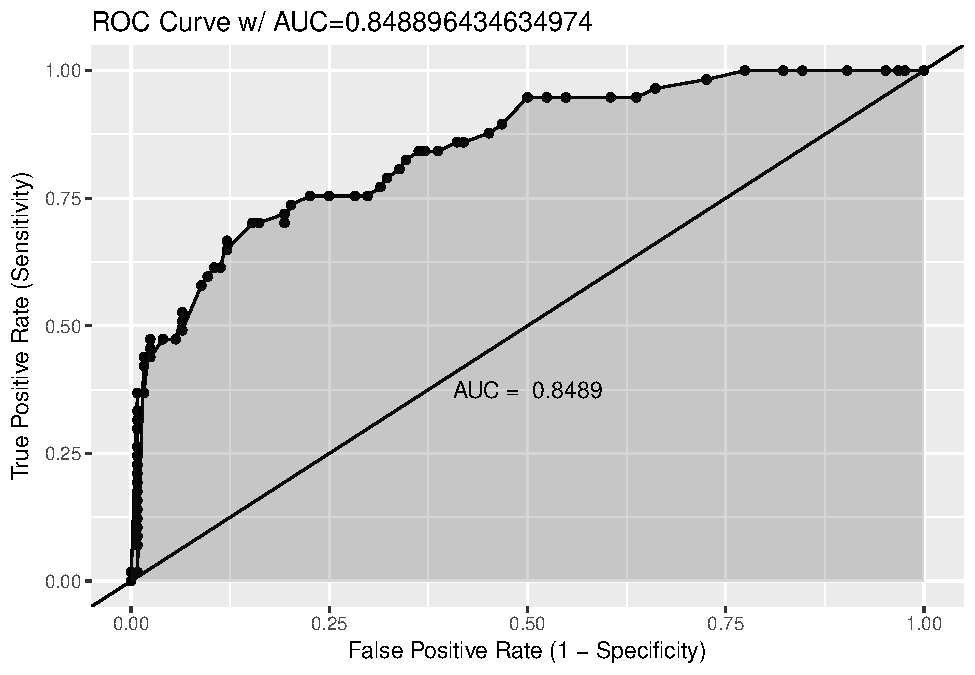
\includegraphics{DATA_621_Homework_2_files/figure-latex/roc-output-1.pdf}

\begin{verbatim}
## 
## [[2]]
## [1] 0.8488964
\end{verbatim}

\section{Task 11}\label{task-11}

Use your created R functions and the provided classification output data
set to produce all of the classification metrics discussed above.

\subsection{Function results}\label{function-results}

\begin{Shaded}
\begin{Highlighting}[]
\KeywordTok{cat}\NormalTok{(}\KeywordTok{sprintf}\NormalTok{(}\StringTok{"}\CharTok{\textbackslash{}n}\StringTok{ %s = %f }\CharTok{\textbackslash{}n}\StringTok{"}\NormalTok{, }\KeywordTok{c}\NormalTok{(}\StringTok{"Accuracy"}\NormalTok{, }\StringTok{"Error Rate"}\NormalTok{, }\StringTok{"Precision"}\NormalTok{, }\StringTok{"Sensitivity"}\NormalTok{, }\StringTok{"Specificity"}\NormalTok{, }\StringTok{"F1 Score"}\NormalTok{), }\KeywordTok{c}\NormalTok{(}\KeywordTok{pred_acc}\NormalTok{(cod), }\KeywordTok{pred_err}\NormalTok{(cod), }\KeywordTok{pred_prec}\NormalTok{(cod), }\KeywordTok{pred_sens}\NormalTok{(cod), }\KeywordTok{pred_spec}\NormalTok{(cod), }\KeywordTok{pred_f1}\NormalTok{(cod))))}
\NormalTok{## }
\NormalTok{##  Accuracy = 0.806630 }
\NormalTok{##  }
\NormalTok{##  Error Rate = 0.193370 }
\NormalTok{##  }
\NormalTok{##  Precision = 0.843750 }
\NormalTok{##  }
\NormalTok{##  Sensitivity = 0.473684 }
\NormalTok{##  }
\NormalTok{##  Specificity = 0.959677 }
\NormalTok{##  }
\NormalTok{##  F1 Score = 0.606742}
\end{Highlighting}
\end{Shaded}

\section{Task 12}\label{task-12}

Investigate the caret package. In particular, consider the functions
confusionMatrix, sensitivity, and specificity. Apply the functions to
the data set. How do the results compare with your own functions?

\subsection{Caret package}\label{caret-package}

\begin{Shaded}
\begin{Highlighting}[]
\NormalTok{confmat <-}\StringTok{ }\KeywordTok{confusionMatrix}\NormalTok{(cod}\OperatorTok{$}\NormalTok{scored.class, cod}\OperatorTok{$}\NormalTok{class, }\DataTypeTok{positive =} \StringTok{"1"}\NormalTok{)}
\NormalTok{confmat}
\NormalTok{## Confusion Matrix and Statistics}
\NormalTok{## }
\NormalTok{##           Reference}
\NormalTok{## Prediction   0   1}
\NormalTok{##          0 119  30}
\NormalTok{##          1   5  27}
\NormalTok{##                                           }
\NormalTok{##                Accuracy : 0.8066          }
\NormalTok{##                  95% CI : (0.7415, 0.8615)}
\NormalTok{##     No Information Rate : 0.6851          }
\NormalTok{##     P-Value [Acc > NIR] : 0.0001712       }
\NormalTok{##                                           }
\NormalTok{##                   Kappa : 0.4916          }
\NormalTok{##  Mcnemar's Test P-Value : 4.976e-05       }
\NormalTok{##                                           }
\NormalTok{##             Sensitivity : 0.4737          }
\NormalTok{##             Specificity : 0.9597          }
\NormalTok{##          Pos Pred Value : 0.8438          }
\NormalTok{##          Neg Pred Value : 0.7987          }
\NormalTok{##              Prevalence : 0.3149          }
\NormalTok{##          Detection Rate : 0.1492          }
\NormalTok{##    Detection Prevalence : 0.1768          }
\NormalTok{##       Balanced Accuracy : 0.7167          }
\NormalTok{##                                           }
\NormalTok{##        'Positive' Class : 1               }
\NormalTok{## }

\CommentTok{# Compare accuracy}
\KeywordTok{all.equal}\NormalTok{(confmat[[}\StringTok{"overall"}\NormalTok{]][[}\StringTok{"Accuracy"}\NormalTok{]], }\KeywordTok{pred_acc}\NormalTok{(cod))}
\NormalTok{## [1] TRUE}

\CommentTok{# Compare sensitivity}
\KeywordTok{all.equal}\NormalTok{(confmat[[}\StringTok{"byClass"}\NormalTok{]][[}\StringTok{"Sensitivity"}\NormalTok{]], }\KeywordTok{pred_sens}\NormalTok{(cod))}
\NormalTok{## [1] TRUE}

\CommentTok{# Compare specificity}
\KeywordTok{all.equal}\NormalTok{(confmat[[}\StringTok{"byClass"}\NormalTok{]][[}\StringTok{"Specificity"}\NormalTok{]], }\KeywordTok{pred_spec}\NormalTok{(cod))}
\NormalTok{## [1] TRUE}
\end{Highlighting}
\end{Shaded}

\section{Task 13}\label{task-13}

Investigate the pROC package. Use it to generate an ROC curve for the
data set. How do the results compare with your own functions?

\subsection{pROC package}\label{proc-package}

\begin{Shaded}
\begin{Highlighting}[]
\KeywordTok{roc}\NormalTok{(cod}\OperatorTok{$}\NormalTok{class }\OperatorTok{~}\StringTok{ }\NormalTok{cod}\OperatorTok{$}\NormalTok{scored.probability, }\DataTypeTok{plot=}\NormalTok{T, }\DataTypeTok{auc.polygon=}\OtherTok{TRUE}\NormalTok{)}
\end{Highlighting}
\end{Shaded}

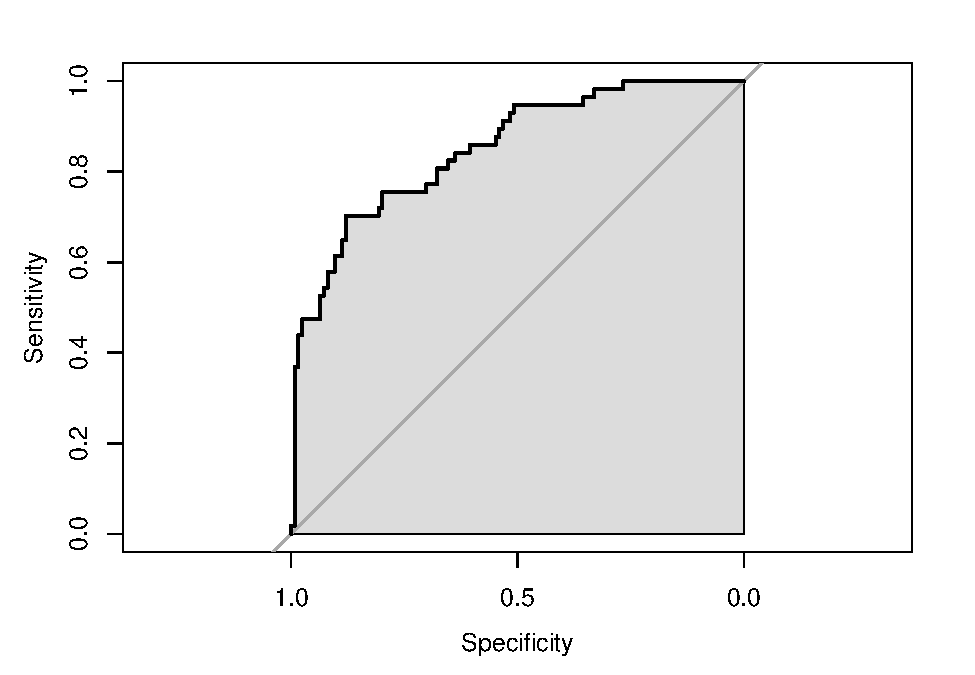
\includegraphics{DATA_621_Homework_2_files/figure-latex/proc-1.pdf}

\begin{verbatim}
## 
## Call:
## roc.formula(formula = cod$class ~ cod$scored.probability, plot = T,     auc.polygon = TRUE)
## 
## Data: cod$scored.probability in 124 controls (cod$class 0) < 57 cases (cod$class 1).
## Area under the curve: 0.8503
\end{verbatim}

The pROC package calculated an AUC of 0.8503, compared to my value of
0.8489, which is within 1\%.

\section{References}\label{references}

\begin{itemize}
\tightlist
\item
  \url{https://www.r-bloggers.com/illustrated-guide-to-roc-and-auc/}
\item
  \url{https://community.alteryx.com/t5/Data-Science-Blog/ROC-Curves-in-Python-and-R/ba-p/138430}
\item
  \url{http://web.ydu.edu.tw/~alan9956/docu/refer/roc_introduction.pdf}
\item
  \url{http://www.saedsayad.com/docs/ROC101.pdf}
\item
  \url{https://www.linkedin.com/pulse/roc-curve-simple-terms-yanchao-liu/}
\item
  \url{https://www.r-bloggers.com/on-calculating-auc/}
\item
  \url{https://stat.ethz.ch/pipermail/r-help/2005-September/079872.html}
\end{itemize}


\end{document}
